% ---------------------------------------------------
% ----- Main document of the template
% ----- for Bachelor-, Master thesis and class papers
% ---------------------------------------------------
%  Created by Claudia Müller-Birn on 2012-08-17. (updated on 2013-04-03)
%  Freie Universität Berlin, Institute of Computer Science, Human Centered Computing (HCC). 
%
\documentclass[pdftex,a4paper,12pt]{scrartcl}   
%
%---------------------------------------------------
%----- Packages
%---------------------------------------------------
%
\usepackage[T1]{fontenc} 
\usepackage[utf8]{inputenc}
%\usepackage[ngerman]{babel} 
\usepackage[english]{babel}  
\usepackage{ae} 
%\usepackage{bibgerm}   
\usepackage[sort]{natbib}

\usepackage[pdftex]{graphicx} 
\usepackage{tikz}
\usetikzlibrary{arrows}
\usepackage{qtree}
\usepackage{fontawesome}
\usepackage{fancyref} 
\usepackage{fancyhdr} % Define simple headings 
\usepackage{xcolor}
\usepackage{url}

%
\usepackage{amsthm}
\usepackage{tabularx}
\theoremstyle{definition}
\newtheorem{definition}{Definition}[section]
\usepackage{pifont}
\usepackage{wrapfig}
\usepackage{caption}
\captionsetup[figure]{format=plain, justification=justified, labelfont=bf}
\usepackage{ragged2e}
\usepackage{overpic} 
\usepackage{hyperref} % turn all your internal references into hyperlinks
%\usepackage[pdfstartview=FitH,pdftitle={<<Titel der Arbeit>>}, pdfauthor={<<Autor>>}, pdfkeywords={<<Schlüsselwörter>>}, pdfsubject={<<Titel der Arbeit>>}, colorlinks=true, linkcolor=black, citecolor=black, urlcolor=black, hypertexnames=false, bookmarksnumbered=true, bookmarksopen=true, pdfborder = {0 0 0}]{hyperref}
% 
% a new command is defined that allows to include an empty page when needed
\newcommand{\blankpage}{
\newpage
\thispagestyle{empty}
\mbox{}
\newpage
}
%
%---------------------------------------------------
%----- PDF and document setup
%---------------------------------------------------
%
\hypersetup{
	pdftitle={<My title>},  % please, add the title of your thesis
    pdfauthor={<Author>},   % please, add your name
    pdfsubject={<<Bachelor thesis>, Institute of Computer Science, Freie Universität Berlin>}, % please, select the type of this document
    pdfstartview={FitH},    % fits the width of the page to the window
    pdfnewwindow=true, 		% links in new window
    colorlinks=false,  		% false: boxed links; true: colored links
    linkcolor=red,          % color of internal links
    citecolor=green,        % color of links to bibliography
    filecolor=magenta,      % color of file links
    urlcolor=cyan           % color of external links
}


%
%---------------------------------------------------      
%----- Settings for word separation  
%---------------------------------------------------      
% Help for separation (from package babel, section 22)):
% In german package the following hints are additionally available:
% "- = an explicit hyphen sign, allowing hyphenation in the rest of the word
% "| = disable ligature at this position. (e.g., Schaf"|fell)
% "~ = for a compound word mark without a breakpoint (e.g., bergauf und "~ab)
% "= = for a compound word mark with a breakpoint, allowing hyphenation in the composing words
% "" = like "-, but producing no hyphen sign (e.g., und/""oder)
%
% Describe separation hints here:
\hyphenation{
% Pro-to-koll-in-stan-zen
% Ma-na-ge-ment  Netz-werk-ele-men-ten
% Netz-werk Netz-werk-re-ser-vie-rung
% Netz-werk-adap-ter Fein-ju-stier-ung
% Da-ten-strom-spe-zi-fi-ka-tion Pa-ket-rumpf
% Kon-troll-in-stanz
}

%---------------------------------------------------      
%----- Settings for title page 
%---------------------------------------------------

\begin{titlepage}

\title{
{\small <Bachelorarbeit> am Institut für Informatik der Freien Universität Berlin}\\
{\small Human-Centered Computing (HCC), AG NBI}\\
[6ex]
{\LARGE Recommender System for Idea-Clustering based on Semantic Similarity of Concepts in Knowledge Graphs }\\
{\normalsize-- Exposé --}}

\author{
{\emph{\normalsize Luka Stärk}}\\
{\normalsize Matrikelnummer: 374532}\\
{\normalsize luka.staerk@campus.tu-berlin.de}\\\\
{\normalsize Betreuer: Michael Tebbe}
}

\date{\normalsize Berlin, \today}

\end{titlepage}

%%%%%%%%%%%%%%%%%%%%%%%%%%%%%%%%%%%%%%%%%%%%%%%%%%%%%%
% The content part of the documentent starts here! %%
%%%%%%%%%%%%%%%%%%%%%%%%%%%%%%%%%%%%%%%%%%%%%%%%%%%%%%

\begin{document}


\maketitle 



\thispagestyle{empty}  % eliminate page number on the title page
\blankpage
%---------------------------------------------------      
%----- Content part  
%---------------------------------------------------

\setcounter{page}{1} % page number is set to "1" otherwise it would be "3"

%\section{Struktur des Exposé}
%Im Folgenden habe ich Ihnen eine generelle Struktur für ein Exposé vorgegeben. Jeder Abschnitt ist mit einer Frage, welchen Inhalt dieses Kapitel abdecken sollte eingeleitet und enthält einige Erläuterungen. Bitte beachten Sie, dass das Layout dieser Vorlage doppelseitig angelegt ist.

\section{Motivation} 
    
%\item In welchem Bereich/Themenfeld bewegt sich Ihre geplante Arbeit?
The research project Ideas2Market explores the innovation process for applications of new technologies. A central task is to generate many ideas, to cover most possible solutions on how to apply the technology. This procedure is implemented using collaborative innovation approaches to crowd-source ideas. These ideas are not yet fully evolved and considered to be on a brainstorming level, in the following they will be referred to as idea sparks. Nevertheless, these idea sparks introduce great variety and creative value because they are created by different persons with diverse backgrounds. Still, finding valuable idea sparks has proven challenging and due to their large number, it becomes unfeasible to check every idea spark manually and to derive benefits from them for advanced ideas. These ideas are evolved by experts in the further process and then become refined and transformed into product opportunities to deploy onto the market as the last step. The project Ideas2Market aims to solve these problems with software support and by researching the human needs in creative processes. The software supported collaborative-ideation process can be described in three phases as illustrated below in Figure \ref{fig:diamond}:

\begin{figure}[h]
    \centering
    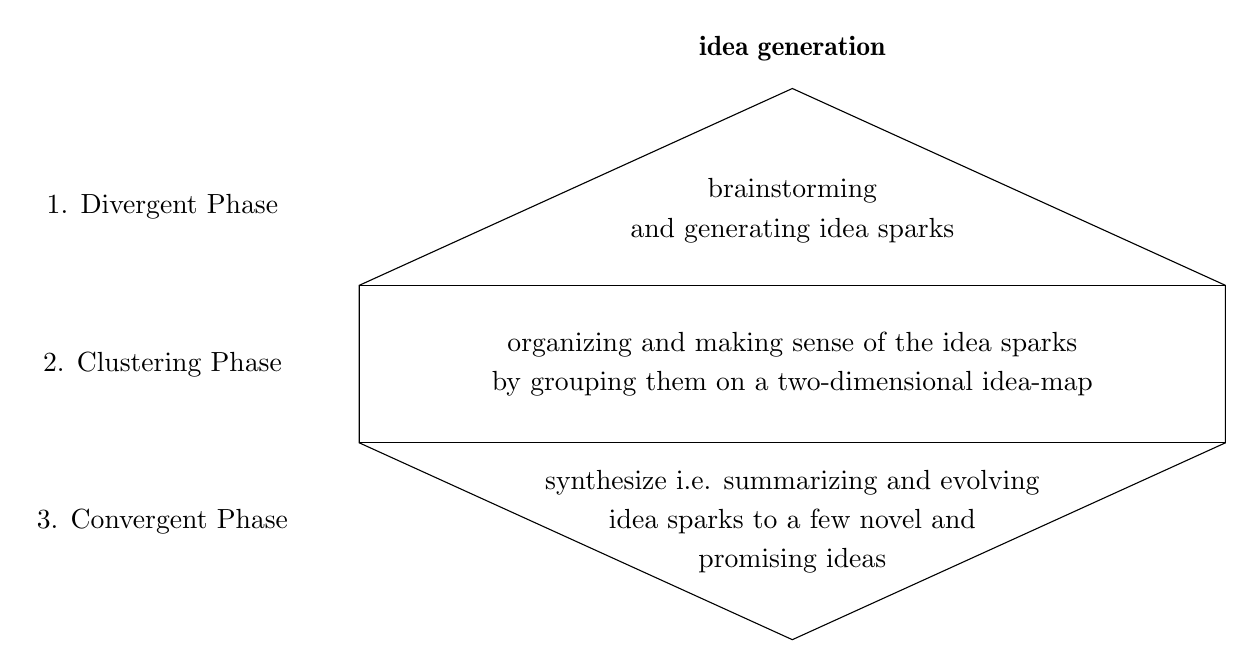
\begin{tikzpicture}
    \draw (5.5, 7) node {\textbf{idea generation}};
    
    \draw (0,3) -- (0,4) -- (5.5,6.5) -- (11,4) -- (11,2) -- (5.5, -0.5) -- (0, 2) -- (0,3);
    \draw (0,4) -- (11,4);
    \draw (0,2) -- (11,2);
    \draw (5.5,5.2) node {brainstorming};
    \draw (5.5,4.7) node {and generating idea sparks};
    \draw (5.5, 3.25) node {organizing and making sense of the idea sparks};
    \draw (5.5, 2.75) node {by grouping them on a two-dimensional idea-map};
    \draw (5.5, 1.5) node { synthesize i.e. summarizing and evolving};
    \draw (5.5, 1) node { idea sparks to a few novel and};
     \draw (5.5, 0.5) node {promising ideas};
    
    \draw (-2.5,5) node {1. Divergent Phase};
    \draw (-2.5,3) node {2. Clustering Phase};
    \draw (-2.5,1) node {3. Convergent Phase};
    \end{tikzpicture}
    \caption{Three Phase Diamond of the Innovation Process \citep{tassoul_clustering:_2007}}
    \label{fig:diamond}
\end{figure}

When clustering, the categories of the emerging clusters and the connections between idea sparks are not always so clear to us. The decision of creating a cluster is based on feeling and intuition and can be reversed any time. During the process an ordering develops and the relationships between idea sparks become more visible, so fare the theory.
Clustering is ought to be beneficial as an activity in acquiring a more profound understanding of the idea-space \citep{siangliulue_ideahound:_2016} and producing more valuable ideas in the Convergent Phase. However, for growing numbers of idea sparks, it becomes more challenging to organize the idea-space and to take into account all potential idea sparks for one cluster. This task can then be monotonous and time-consuming. My thesis is about counteracting this problem and increasing efficiency in the clustering process.% with a recommender system that proposes idea sparks based on the selection of content, that can either be an idea spark or single concepts.
    %Recommender System? 
   
    %\item Erläutern Sie kurz, in welchem Themenbereich Ihre Arbeit angesiedelt ist. Wo werden Sie einen Beitrag leisten?
    
    %\item Nutzen Sie bei den Erläuterungen die Ihnen bereitgestellte Kurzaufgabenstellung.

\section{Thematic Classification of Thesis}

    %Welche Artikel/Literatur sind/ist relevant für diese Arbeit?
    
        % Computing  Semantic  Similarity  of  Concepts  in Knowledge Graphs \citep{zhu_computing_2017}
    

%\item Bitte geben Sie die relevanten Inhalte der Artikel kurz wieder.
    %TODO: 
    %\item Das Ausarbeiten von ausgewählter Literatur bzw. verwandten Arbeiten hilft Ihnen, Ihre Ziele im folgenden Abschnitt zu definieren. Daher ist eine Auseinandersetzung mit der Literatur von Beginn an notwendig, wenn es zu diesem Zeitpunkt noch nicht erschöpfend sein muss.
\subsection{Orchard Clustering Application}
    In the research project Ideas2market the Clustering Web-Application Orchard has been developed to support the second and third phase of the ideation process (see Figure \ref{fig:orchard} for the clustering step). Orchard is inspired by the IdeaHound project \citep{siangliulue_ideahound:_2016} and a tool for creative ideation to effectively synthesize ideas from numerous idea sparks. For the clustering phase, the user can drag and drop ideas from the \textit{Spark Stack} on to the whiteboard. To create clusters or add to an existing cluster, the user drops one idea spark on to another or an existing cluster. The user can inspect an idea spark in detail by clicking on it. In that case the complete description and labels of the idea spark are displayed in the right column (see Figure \ref{fig:orchard} (5)).
     
    \begin{figure}
        \centering
        \begin{overpic}[width=15cm]{pics/RS-O.png}
        \put(2,22){\ding{172}}
        \put(2,44){\ding{173}}
        \put(49,40.5){\ding{174}}
        \put(31.5,38){\ding{175}}
        \put(86,45){\ding{176}}
        \put(39,37){\faHandPointerO}
        \end{overpic}
        \caption{Clustering view of the Orchard interface, where the recommender frame (1) displays similar idea sparks to \textit{SPARK 2} (4) from the Cluster named \textit{PET} (3) with two idea sparks. (5) The right column displays the full content of the idea spark, that the user selects by mouse click and further the caption is set in bold, see \textit{SPARK 2} (4).
        }
        \label{fig:orchard}
    \end{figure}
    
\subsection{Supporting Effective Collective Ideation at Scale}
    One solution to increase efficiency in synthesizing ideas is to introduce a predefined idea-map, where the idea sparks are organized in clusters by similarity score \citep[124]{siangliulue_supporting_2017}. In addition, it is easier for the user to internalize the idea-space and thus interact more with rare ideas \citep{siangliulue_supporting_2017}, which is a benefit in quality because ideas are often mundane or repetitive \citep{siangliulue_ideahound:_2016}. Then again, the user is more fixated on the categories that were given by the clusters and might miss other possible syntheses that would have been created without the suggested clusters \citep{siangliulue_supporting_2017}. To increase efficiency in the clustering phase and prevent fixation on given categories I propose an idea recommender system, as shown in Figure \ref{fig:orchard} on the left (1), for the Orchard Application. So that the user can walk through the idea sparks lead by his changing interest of categories, clusters, and topics. 
    
\subsection{Recommender System}
Recommender systems (RS) became popular in commercial platforms like Online Shops and Streaming Services and is a subclass of information filtering system, that predicts the user's interest for specific content. To navigate successfully through large information spaces RSs have been an important tool. There are different types of RSs that are often combined into hybrids. One of the most prominent types is collaborative filtering where predictions are derived from the behavior of other users. Another approach is content-based filtering, which is based on the description of an item. Through the user's interaction history with the RS, a classifier of his preferences is learned to predict the user's interest in the following interaction. 
Knowledge-based is a third type, that provides recommendations through reasoning about which items match the user's requirements. Thus it requires specific knowledge about the items (e.g. an underlying ontology or data-model with many properties) and the user's requirements. To map these requirements to the ranking of items, recommendation criteria have to be defined. It can cause a knowledge bottleneck due to considering only the explicit knowledge in the RS.
But in contrast to the first two types, the knowledge-based advantage is that it has no "cold-start" problem, where a lot of users data and ratings are required to provide accurate recommendations and gain implicit knowledge about users and items. 

In the scope of my bachelor thesis, an RS will be developed for the clustering application Orchard to recommend idea sparks that are similar to a selected spark. The similarity measures of the RS are based on a single idea spark or one concept of one spark. In this manner, one can specify further the recommendations made for other idea sparks. 

The RS in Orchard is knowledge-based. To provide recommendations the user's requirements are specified by selecting idea sparks and concepts of the user's current interest. Criteria for the RS is the semantic similarity of concepts. The Wikidata ontology contains the concepts of idea sparks and supplies the necessary information to apply measurements as recommendation criteria.
    %Why Knowledge Graph-based? 
\subsection{Knowledge Graph}
    For the similarity measures, I use the relations between defined concepts in a Knowledge Graph (KG). In the context of semantic web and linked data many Knowledge Graphs like DBpedia and Wikidata, are freely accessible and gain increasing popularity. KGs are semantic networks where relations between concepts and entities are recorded as triples (subject, predicate, object). These Information Networks are used for different Natural Language Processing and Information Retrieval tasks like word sense disambiguation, topic modeling and Question Answering \citep{nastase_topic-driven_2008}. 
    Semantic similarity is a metric to measure the similarity of concepts in the KG through their hierarchical relations \citep{zhu_computing_2017}. The advantage of this approach is that the similarity becomes interpretable when looking up the connecting path or the lowest common ancestor concept in the directed acyclic graph. In statistical approaches, this information is more difficult to extract because the semantic relationships of concepts are not accessible as facts, like in a KG, rather as distances in high-dimensional spaces.
    Wikidata records more than 69 million items\footnote{https://www.wikidata.org/wiki/Wikidata:Statistics} and covers most of the real-world entities and is considered useful as KG in this approach. 

\subsection{Similarity of Concepts}

\begin{figure}
\tikzset{edge/.style = {->,> = latex'}}

    \centering
    \begin{tikzpicture}
    \node (1) at (5,10.5) {entity};
    \node (2) at (5,9.5) {vehicle};
    \node (3) at (3,8) {motor vehicle};
    \node (4) at (2,7) {car};
    \node (5) at (3,7) {bus}; 
    
    \node (6) at (6, 8.5) {two-wheeler};
    \node (7) at (7, 7.7) {bicycle};
    \node (8) at (8, 7) {race-bike};
    \node (9) at (5, 7) {motor-bike};
    
    \node (10) at (10, 8.5) {aircraft};
    \node (11) at (10, 7.5) {airplane};
    
    \node (12) at (10, 10) {artificial entity};
    
    \draw[edge] (1) to (12);
    
    \draw[edge] (2) to (10);
    \draw[edge] (10) to (11);
    
    \draw[edge] (2) to (6);
    \draw[edge] (6) to (7);
    \draw[edge] (7) to (8);
    \draw[edge] (6) to (9);
    \draw[edge] (3) to (9);
    
    \draw[dashed,->] (1) to (2);
    \draw[edge] (2) to (3);
    \draw[edge] (3) to (4);
    \draw[edge] (3) to (5);
\end{tikzpicture}
    \caption{Part of the Knowledge Graph from Wikidata}
    \label{fig:kg}
\end{figure}

In the field of Semantic Similarity, there are several metrics to measure the similarity of terms, concepts and instances.
Measuring semantic similarity divides up into mainly corpus-based and knowledge-based approaches. Corpus-based semantic similarities metrics use statistical relations of words in a large text collections. Two words are similar, when their surrounding text context is similar. This approach relies on the occurrence of words and ignores the different meaning a word can have, namely word sense disambiguation \citep{zhu_computing_2017}. 
In contrast, knowledge-based semantic similarity metrics, measure similarities between defined concepts in a KG. The most simple similarity metric takes the shortest path distance between two concepts and transforms it into a score $s \in [0,1]$. For two concepts $c_i,c_j$ let $length(c_i,c_i)$ denote the shortest path between $c_i,c_j$ then the similarity is calculates as 
\begin{equation}
    sim_{path}(c_i,c_j) = \frac{1}{1+length(c_i,c_j)}.
\end{equation}

Another importend measurement that occurs in corpus-based as well as in knowledge-based metics is the Information Content (IC). The IC of a concept determines how abstract or specific a concept is and how much information the entities of a concept share, so intuitively more abstract concepts hold lower IC values and more specific ones higher values of IC. There are different ways of measuring the IC, \citet{zhu_computing_2017} propose the following definitions: 
\begin{definition}{Information Content corpus-based:}

Let $c_i$ be a concept, given a large general text-corpus $Prop(c_i)$ is the probability to encounter a word from the set of $words(c_i)$ that are subsumed or associated with $c_i$. $Prob(c_i)= \frac{\Sigma_{w\in words(c_i)} count(w)}{N}$, where $N$ is the total number of concepts observed in the text-corpus. The Information Content can be quantify as negative the log likelihood $-log_e Prob(c_i)$ \citep{resnik_using_nodate}, then the $IC_{corpus}(c_i) = -log_e Prob(c_i)$, so intuitively the IC of concept $c_i$ increases when the probability decreases and if there would be one concept subsumming all other concepts its IC would be $0$. 
\end{definition}
\begin{definition}{Information Content graph-based:}

Let $c_i$ be a concept, then the $IC_{graph}(c_i) = -log_e Prob(c_i)$, where the $Prob(c_i) = \frac{count(entities(c_i))}{N}$ and $entities(c_i)$ is a set of entities with type $c_i$ in the KG and $N$ is the total number of entities in the KG. 
\end{definition}

%Other populare measures for semantic similarity such as considering the $depth(c) = length(c,root)$ of a concept $c$ in the KG, that have shown good result. The assumption is that concepts with higher depth are more specific and thus are similar to the IC measurements. Structural metrics compare the neighborhood or upper ancestral graph of concepts. 

The publication \textit{Computing  Semantic  Similarity of  Concepts in Knowledge Graphs} of \citet{zhu_computing_2017} discusses different metrics of concept similarity in Knowledge Graphs and compares them to their approach \textit{wpath} with gold standard data sets of human-judged similarity in meaning. Their metric $wpath$ for measures of similarity considers shortest-path length between two concepts in the Knowledge Graph and the Information Content (IC) of their least common subsumer (LCS). The LCS of two concepts is the most specific ancestral concept that is shared by both concepts. Therefore the LCS is the one with the highest IC among the shared ancestors. E.g in the KG shown in Figure \ref{fig:kg}, the concept \textit{two-wheeler} is the LCS of \textit{motor-bike} and \textit{bicycle}, and not \textit{vehicle}, because it is more abstract. \citep{zhu_computing_2017} define the semantic similarity methode as 
\begin{equation}
    sim_{wpath(c_i,c_j)} = \frac{1}{1+length(c_i,c_j) \cdot k^{IC(lcs)}},
\end{equation}

where the parameter $k \in (0,1]$ weighs between IC of the LCS and the path length of two concepts. If $k = 1$ the IC has no influence to the path length. Otherwise the IC weights the path length, so that concepts with the same path length but different LCS can have different similarities. E.g. $car$ and $bus$ are more similar than $two-wheeler$ and $aircraft$, though for both pairs the path length equals two, as shown in Figure \ref{fig:kg}. 

\subsection{Human-Centered}

\begin{wrapfigure}{R}{0.35\textwidth}
    \centering
    \begin{overpic}[width=0.33\textwidth]{pics/rs-and-weight.png}
    \put(35,10){\ding{172}}
    \end{overpic}
    \caption{Recommender System with highlighted concepts of different saturation depending on similarity to the selected object. (1) Slider to change weight in $wpath$ metric.}
    \label{fig:rs}
\end{wrapfigure}

In the field of machine learning and beyond, human-centered approaches have gained extensive attention. As machine learning discover relations and patterns in data instead of programming explicit rules, the solution may reflect the bias and incompleteness of the used data and contain uncertainties. 
Viewing the problem through the human lens and considering human needs, ensures that the problems stay's grounded. 

The mentioned concerns apply to this thesis as well. The RS is based on knowledge graph states and other assumptions such as the metric $wpath$ and its parameter $k$. When interacting with a so-called intelligent-system, the user will naturally form a mental model of it and adjust interaction and behavior to the assumptions being made. E.g. the RS in Orchard may respond with unrelated idea sparks for some concepts so that the user will try to identify and then avoid using these concepts. So when the user has a good mental model of the system, the interaction is more effective. Which gives reason to consider interpretability and transparency of the system when thinking about the User Interface. Furthermore, leaving tasks to the user, that the user performs best, makes the system more adaptive and gives the user the feeling of being in control, so that the user will be more likely to interact with the system \citep{abdul_trends_2018}. E.g in the Orchard application the user selects the concept that is most interesting of an idea spark, to be more specific in what he or she is interested in. Another feature for the User Interface will be a Slider in a range, as shown in Figure \ref{fig:rs} (1), to change the $k$-parameter, weighting between the impact of path length and Information Content of the LCS. Thus the user can experiment and get an idea which weight leads to good results. For more transparency and a better understanding of the RS, the idea sparks in the recommender frame are visualized with highlighted concepts as well, as Figure \ref{fig:rs} illustrates. In which the color saturation depends on the similarity to the selected idea spark or concept. Thereby it becomes easier for the user to create a mental model of the RS and to understand why a certain idea spark is ranked as most similar.

\section{Goal} 
    %\item Welche Ziele werden mit der Arbeit verfolgt? Und welche zentralen Fragen lassen sich daraus ableiten?
    
\begin{wrapfigure}{R}{0.35\textwidth}
\centering
\begin{overpic}[width=0.33\textwidth]{pics/spark.png}
\put(20,57){\faHandPointerO}
\end{overpic}
\caption{Spark with highlighted concepts}
\label{fig:spark}
\end{wrapfigure}

The goal of my thesis is to improve the clustering process in the Orchard application with a recommender system. Thus the user should interact more with rear and valuable idea sparks and cluster more effectively without fixation on predefined categories. To apply the RS, concept similarity is calculated for all concepts extracted from 60 goldstandard idea sparks. The proposed metric $wpath$ of \citet{zhu_computing_2017} combines meaningful sematic similarity measures for the application on a Wikidata KG and has shown outperforming results for the DBpedia ontology. As the Wikidata KG is especially large and complex it is of interest answering, how well semantic similarity metrics performe on such KGs compared to others. 
Given the measures of similarity between concepts, the similarities between concepts and ideas, and the Word Mover's Distance between ideas are calculated, these are the measurements needed to integrate the recommender system into the Orchard clustering application.

In Orchard, as Figure \ref{fig:spark} illustrates, the user can click on an idea spark or a highlighted concept of it's description to select the content, based on that idea sparks with similar concepts are recommended. The recommended idea sparks are displayed in the recommender frame sorted by highest similarity and the user can scroll through and drag them onto the whiteboard (see Figure \ref{fig:orchard} (1)).


    
    %\item Die Ziele sollten so spezifisch wie möglich sein. Das hilft Ihnen im Verlauf der Umsetzung zu prüfen, ob Sie Ihre Ziele erreichen konnten.
%\end{itemize}

\section{Planned Procedure}
%\begin{itemize}
    %\item Welche einzelnen Aktivitäten müssen umgesetzt werden, um die Fragen zu beantworten und das Ziel der Arbeit zu erreichen?
    The Procedure for my thesis is divided into three substantial parts: implementation, integration into the Orchard application and the validation of the results. 
    \subsection{Implementation}
    
    The requirement for the input data of idea sparks is that the concepts of the idea descriptions are assigned to Wikidata items. In prepossessing all stop-word concepts, such as "I, my, You,\dots" and concepts that do not connect to get KG are excluded.
    
    The following functions will be implemented to apply the $wpath$ metric for concept similarity.
    \begin{itemize}
        \item A function to generate a subgraph of the Wikidata Knowledge Graph.
        The subgraph is extracted with \textit{SPARQL} queries to the \textit{Wikidata} SPARQL-endpoint. The set of concepts that occur in the idea sparks build the bottom child layer of the KG. All existing connections in Wikidata from each idea-concept to $entity$, over the three predicates \textit{subclass of (P279), instance of (P31), part of (P361)} are extracted for the KG. In which $entity$ is the highest concept in the hierarchy of the Wikidata KG. (done)
        \item A function to resolve an directed graph into an directed acyclic graph (DAG). (done)
        \item A function to calculate the Information Content graph-based for all concepts in the DAG, over the edges \textit{subclass of (P279), instance of (P31)}. 
        \item A function that finds the least common subsumer for all pairs of two concepts in the DAG. (done)
        \item A function that calculates the all-shortest ancestral distance in the DAG, i.e. the shortest path between two nodes over their LCS. (done)
    \end{itemize}
    
    For the similarity measures from a concept to an idea spark, I will implement a function that returns the idea sparks which contain the concepts that are most similar to the concept given as input. 
    
    To calculate the similarity between idea sparks I will implement the word mover's distance (WMD) \citep{kusner_word_nodate} based on the similarity of their concepts. 
    
    \subsection{Integration into Orchard}
    
    For the Orchard application, I will integrate the similarities, provided by the implementation for a given data-set of idea sparks, into the database of Orchard. 

    For the client-side I will add a recommender frame (see Figure \ref{fig:orchard} (1)) and highlight the annotated concepts in the idea-description in the detail view (see Figure \ref{fig:orchard} (5)). When the user hovers over any idea spark on the whiteboard the concepts in the description become highlighted as well (see Figure \ref{fig:spark}). The highlighted concepts are clickable and a function updates the recommendations for the new source. 

    A React Component will be programmed that displays the idea sparks with highlighted concepts, with different color saturation, depending on the similarity to the selected object, see Figure \ref{fig:rs}.
    
    \subsection{Validation}
    The validation consists of the following three steps:  
    \begin{enumerate}
        \item To validate the measures of concept similarity, the implementation of $wpath$ will be compared to the \textit{R\&G} dataset \citep{rubenstein_contextual_1965} of human-judged word similarity and the results of the implementation of $wpath$ from \citet{zhu_computing_2017}. \textit{R\&G} is a widely used dataset containing human assessment of word similarity for 65 word-pairs of common English nouns.
        \citet{zhu_computing_2017} uses the same dataset for $wpath$ with corpus-based IC and graph-based IC with the DBpedia ontology. This comparison will be done for different parameter $k \in (0,1]$ for $wpath$, to optimize the measurements for \textit{R\&G}. 
        \item To find the best weight $k$ between path length and IC for the Wikidata KG, the $wpath$ similarity will be applied on several idea-concepts for different parameters $k \in (0,1]$.
        \item  As the last step, the recommender system will be tested with Orchard on a qualitative level with three or more persons who are familiar with the clustering process, to evaluate the research question, if the recommender system in Orchard is a helpful feature to effectively find clusters and creating a satisfying result. 
    \end{enumerate}
    
    
    
   
    
    
    
    %\item Aus den Fragen (vorheriger Abschnitt) können Sie dann gut Aktivitäten ableiten, die Ihnen helfen, Ihre weitere Arbeit zu strukturieren.
    
    
%\end{itemize}

\section{Technical Implementation}
%\begin{itemize}
    %\item Mit welchen softwaretechnischen Hilfsmitteln soll die Arbeit realisiert werden?
    
    The software is realized in python and  the Knowledge Graph is extracted from Wikidata.
    For the calculation of the corpus-based IC, the implementation of \citet{zhu_computing_2017} is used. 
    The Interface of the recommender system in Orchard is implemented in JavaScript, React and Redux.  
    
%\end{itemize}

\section{First Schedule}
\renewcommand{\arraystretch}{1.5}
\begin{tabularx}{\textwidth}{lX}
28. October & Implementation of $IC_{graph}$\\
6-10. November & Presentation of the thesis topic at HCC\\
8. November & Find a primary supervisor from TU-Berlin.\\
8. November & Annotate and connect $R\&G$ concepts to Wikidata\\
15. November & Registration of the bachelor thesis at the TU-Berlin \\
15. November & Implementation of $wpath$\\
20. November & Validation of $wpath$ and comparison with dataset of \citet{rubenstein_contextual_1965} and implementation of \citet{zhu_computing_2017}.\\
30. November & Implementation of $WMD$ for similarity measures. \\
4. December & Test concept similarity implementation of $wpath$ for Wikidata, to select best parameter $k$. \\
20. December & Finish technical implantation, take measurements for similarity.\\
30. December & The recommender system is integrated into Orchard for gold standard ideas. \\
3. January & Discussion of the results with Prof. Dr. Claudia Müller-Birn, Michael Tebbe and Maximilian Mackeprang.\\
25. January & The thesis are written, time for correction.\\
15. February & Submission of the bachelor thesis\\
\end{tabularx}


%\section{Wie geht es nach dem Exposé weiter?}

%Nachdem die Phase der Exposé-Erstellung abgeschlossen ist (das kann bis zu drei Iterationen dauern), können Sie mit der Erstellung der eigentlichen Abschlussarbeit beginnen. Bitte nutzen Sie die Inhalte des Exposés gleich als inhaltlichen Rahmen für die Arbeit (vor allem in Kapitel 1). Ihnen wird wieder eine \LaTeX Vorlage zur Verfügung gestellt. In dieser Vorlage finden Sie wieder viele Informationen und Hilfestellungen zur Erstellung der Arbeit. Sie sollten nun Ihre Arbeit anmelden. Das entsprechende Formular finden Sie auf den Institutsseiten (\href{http://www.mi.fu-berlin.de/inf/stud-bioinf/downloads/Anmeldung_zur_Bachelorarbeit_2010.pdf}{Link}).Bitte bringen Sie das ausgefüllte Formular zu einer unserer Sitzungen mit. Ich unterschreibe es und leite es weiter. Nun sollten Sie auch bald darüber nachdenken, wer der Zweitgutachter Ihrer Arbeit sein könnte. Ich berate Sie dabei gern. 

%Viele weitere, nützliche Informationen finden Sie in der Prüfungsordnung Ihres Studiengangs. Bitte lesen Sie den Sie betreffenden Absatz im Anhang (\ref{sec:bachelor}). 
%---------------------------------------------------
%----- Bibliography
%---------------------------------------------------
\newpage
\phantomsection
\addcontentsline{toc}{chapter}{Literatur}   % headline
\bibliographystyle{plainnat}  % citation style
\bibliography{biblography} % bib file

\newpage 
\section*{Anhang I: Auszug Prüfungsordnung Bachelor}
\label{sec:bachelor}     
\begin{figure}[!h]
	\centering
		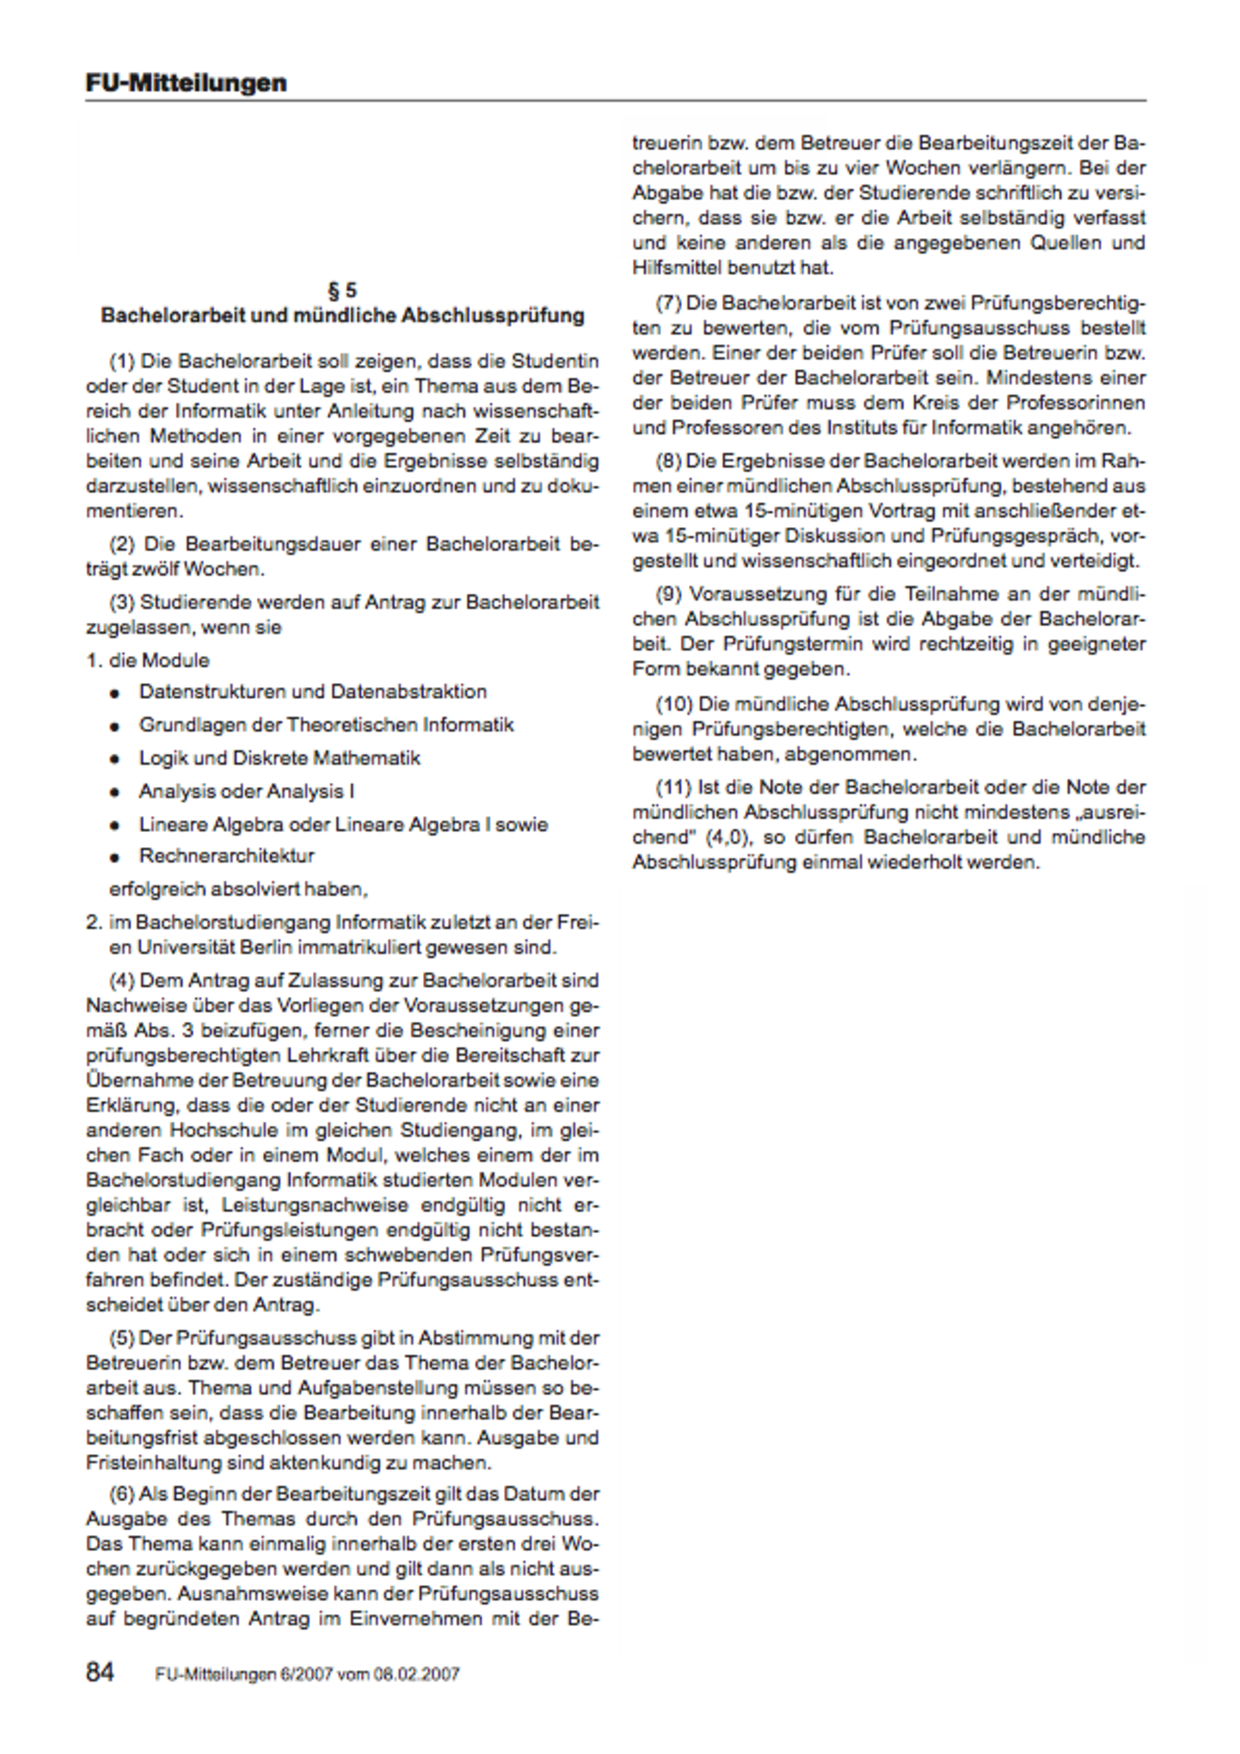
\includegraphics[width=0.8\textwidth]{pics/Auszug_Bachelor_Pruefungsordnung.pdf}
	\caption{Auszug Prüfungsordnung Bachelor} 
\end{figure}

\end{document}
